\documentclass[12pt,a4paper,]{adreport}
\usepackage[T1]{fontenc}
\usepackage{lmodern}
\usepackage{amssymb,amsmath}
\usepackage{ifxetex,ifluatex}
\usepackage{lscape}
\usepackage{fixltx2e} % provides \textsubscript
% use upquote if available, for straight quotes in verbatim environments
\IfFileExists{upquote.sty}{\usepackage{upquote}}{}
\ifnum 0\ifxetex 1\fi\ifluatex 1\fi=0 % if pdftex
  \usepackage[utf8]{inputenc}
\else % if luatex or xelatex
  \ifxetex
    \usepackage{mathspec}
    \usepackage{xltxtra,xunicode}
  \else
    \usepackage{fontspec}
  \fi
  \defaultfontfeatures{Mapping=tex-text,Scale=MatchLowercase}
  \newcommand{\euro}{€}
\fi
% use microtype if available
\IfFileExists{microtype.sty}{\usepackage{microtype}}{}
\usepackage{longtable,booktabs}
\usepackage{graphicx}
% Redefine \includegraphics so that, unless explicit options are
% given, the image width will not exceed the width of the page.
% Images get their normal width if they fit onto the page, but
% are scaled down if they would overflow the margins.
\makeatletter
\def\ScaleIfNeeded{%
  \ifdim\Gin@nat@width>\linewidth
    \linewidth
  \else
    \Gin@nat@width
  \fi
}
\makeatother
\let\Oldincludegraphics\includegraphics
{%
 \catcode`\@=11\relax%
 \gdef\includegraphics{\@ifnextchar[{\Oldincludegraphics}{\Oldincludegraphics[width=\ScaleIfNeeded]}}%
}%
\ifxetex
  \usepackage[setpagesize=false, % page size defined by xetex
              unicode=false, % unicode breaks when used with xetex
              xetex]{hyperref}
\else
  \usepackage[unicode=true]{hyperref}
\fi
\hypersetup{breaklinks=true,
            bookmarks=true,
            pdfauthor={},
            pdftitle={},
            colorlinks=true,
            citecolor=blue,
            urlcolor=blue,
            linkcolor=magenta,
            pdfborder={0 0 0}}
\urlstyle{same}  % don't use monospace font for urls
\setlength{\parindent}{0pt}
\setlength{\parskip}{6pt plus 2pt minus 1pt}
\setlength{\emergencystretch}{3em}  % prevent overfull lines
\setcounter{secnumdepth}{5}

\author{}
\date{}

\begin{document}

{
\hypersetup{linkcolor=black}
\setcounter{tocdepth}{2}
\tableofcontents
}
\chapter{Introduction}\label{introduction}

Distribackup is an open-source file synchronisation tool designed around
the twin principles of decentralisation and one-to-many updates. It aims
to function as autonomously as possible, reducing required technical
knowledge as much as possible in order to make it a viable solution for
data backup for as wide an audience as possible.

\section{Overall Aim of the Project}\label{overall-aim-of-the-project}

Distribackup aims to allow normal technology users to create and manage
highly fault-tolerant backups of archival data (such as family photos,
videos or genealogical documents) without relying on expensive dedicated
hardware or transient cloud services.

As such, it aims to require as little user intervention as possible in
normal use, and to be able to function normally with the less than ideal
parameters for backup that occur in normal domestic environments. This
includes being able to handle poor network connections, keeping
infrequently used machines up-to-date, and accidental data loss.
Generally the aim to either route around or repair damage from the
common mishaps that can affect backed up data over a long period of
time.

\section{Problem Description}\label{problem-description}

The last 5 years have seen a turning point in the backup of personal
data; having been the domain of specialised hobbyists and particularly
diligent computer users who don't exist in every family, corporate
custody of data has provided a convenient outlet to the increasing
pressure of data security.

In this report I argue that data backed up with for-profit organisations
is far less secure than the significant dedicated server infrastructure
invested in `the cloud' would suggest, due to various long-term factors
including company buyouts and political or governmental intervention.

It has also been argued in recent years that the major challenge in
long-term data preservation is not in preserving the bits themselves,
but guarding against bit-rot. Actually being able to read the file
format the data was originally stored in 20 years later can be
difficult.\cite{fosdem15rice}.

This problem can badly affects closed file formats owned by a single
entity. If that company goes bankrupt, is bought out, or for some other
reason discontinues its support of the file format, then no-one else can
continue to make new software that can read data stored in that format,
without significant effort spent to reverse-engineer the format.
Creation of new reading software may even be actively prevented, if the
software is being suppressed after a hostile takeover, or for other
corporate-political reasons. Without new reader software, as the
operating system the reader originally ran on becomes obsolete and is
replaced, and as the hardware architecture the operating system ran on
becomes obsolete and is itself replaced, so the file format becomes
unreadable without relying on ancient hardware, which may itself
physically fail.

This project aims to put the possibility of archival storage within
reach of the general public, unfettered by reliance on changing hosting
agreements or closed-source software obsolescence.

\section{Project Goals}\label{project-goals}

The main objectives of this project are to:-

\begin{itemize}
\itemsep1pt\parskip0pt\parsep0pt
\item
  Develop a distributed backup syncing program, autonomous enough for
  non-technical users to be able to use, and efficient enough to run on
  domestic computer hardware;
\item
  Design and implement an efficient file synchronisation protocol to
  support this;
\item
  Design and implement a new serialisation suite which is both efficient
  for our purposes and simple to work with

  \begin{itemize}
  \itemsep1pt\parskip0pt\parsep0pt
  \item
    Write a language-agnostic specification
  \item
    Implement the specification in Java
  \end{itemize}
\end{itemize}

Data are stored on physical media which are vulnerable to damage, loss
or corruption. CDs are damaged by heat, light and wear and tear. When
this storage fails (mobile phones are lost, old PCs break down or are
replaced due to age, without sufficiently diligent data transferral),
often the user unwittingly throws away or loses many years of
irreplaceable data.

Lost laptops and pen drives cause frequent loss of important data. Old
PCs being replaced cause families to throw away accumulated personal
data, without realising what is stored locally rather than on the
Internet -- lack of understanding causes further personal data loss upon
hardware failure.

The backup strategy often lauded as the most prudent follows the 3-2-1
strategy: 3 copies, on 2 different storage media, 1 off-site
backup.\footnote{``Backups with the 3-2-1 rule''
  (http://blog.wisefaq.com/2010/01/05/backups-with-the-3-2-1-rule/)
  (accessed 25/06/2014)} This is an ideal, but is extremely difficult
for a home user to set up and maintain, without corporate resources at
their disposal. For instance, how can one set up backups in different
locations? And how can one keep off-site copies synced?

This project aims to answer these questions with a software solution,
reducing the risk of data loss for families (and other groups with an
interest in long-term data preservation) due to lack of sufficient
knowledge and/or funds for more thorough backup solutions, without
relying on a third party service that has ulterior motives.

\section{Main Project Features}\label{main-project-features}

Distribackup watches a directory, keeping its contents synced with
copies of the data on other computers. Because the authoritative server
broadcasting updates is likely to be a low-end machine, update data will
be shared among subscribed peers. In order to expedite large file
transfers (which are likely in the primary use case), a differencing
algorithm will be used to only send pieces of files that have changed
since an update.

Having described the problem this software attempts to solve and why it
is needed in this chapter, the Background chapter looks at related work,
talking about how existing solutions could be improved upon for the
identified problem, and how this project builds on this work. In the
Design chapter, the proposed software is described in greater detail
order to complete the bare-bones implementation offered here; continuing
by laying out the sub-components of the software, their purposes, and
how they fit together to complete the end goal. The methodology will
then be explained, describing what software development techniques will
be used during the project. This will lead into the proposed evaluation
methodology, and how research will be carried out.

The expected time-line for this work will then be described in detail,
accompanied by a Gantt chart showing this visually. The report will then
finish by listing the resources required in order for it to be
completed, and a list of references used.

\chapter{Background}\label{background}

Computers have made it convenient and useful to store all our important
family data digitally. Family photos, videos, genealogy records, old
family recipes all take far less physical space on a disk, and can be
copied easily for interested parties, such as relatives.

In the past, any further backups made after transfer to computer would
be in the form of digital media. Digital tape generally required too
high an investment for home users, so writable CDs and DVDs became
common home backup media. Some even dedicated a hard-drive to off-line
storage of the data: the drive would only be switched on when data
needed to be added, deleted or retrieved.

However, stored digital data is at a higher risk of complete loss
(flooding, fire and theft being the most often mentioned) than physical
data, due in part to creating a single point of failure, and also
partially due to the Digital Cliff Effect, which means that digital data
becomes completely unreadable when data integrity drops below
80\%{[}\^{}cliffEffect{]}.

Originally discovered as a property of digital TV transmission, the
Cliff Effect can also come into effect on a hard drive or tape drive
which has remained switched off for long periods. Electromagnetic
interference can corrupt portions of the stored data; left alone long
enough, this can make data unrecoverable. Most families have neither the
resources nor the technical background at their disposal to preserve
their family's unique data long-term. Lay users often have little or no
idea about where or how their data is stored (on their computer or on
the Internet), whether it is safe and whether their own rights to it
have been waived.

Companies have therefore emerged which make it easy to back-up data

Data storage has become a seemingly `solved problem' the responsibility
of storing backup data has been handed over to corporate groups, who
leverage their existing massive server infrastructure (or
subcontractors) to reduce the time and effort spent by ordinary users to
back up their data. The concept of the `cloud' arose as a further
psychological reinforcement of the harmlessness and safety that these
data-centres provide.

In reality, data storage technologies (and the companies running them)
are much more fallible. Corporations want data because it is a resource,
which can be analysed or sold for profit. Information of this type is
now available at such scale that new psychological techniques have been
devised to encourage users to share more personal information, such as
gamification (``Your profile is only 30\% complete''). This data has
value, and drives the economy of the modern web.

It is almost impossible to reverse corporate control over an area of
human interest -- especially an unregulated one with broad scope for
profit from low-level exploitation en masse. However some things have
been shown to be easier to fix than others. The Open Source movement has
shown that by initially appealing to users' greed by offering something
for which they would otherwise have to pay money for free, it is
possible to draw non-technical users away from for-profit services. The
effectiveness of doing this is also strongly influenced by the
presentation and appeal of the software, which modern businesses have
evolved to take very seriously, creating an entire field called `brand
management'.

\section{Summary of Technical Problems and
Approaches}\label{summary-of-technical-problems-and-approaches}

More than ever before there is a need for long-term backup software
which is accessible for everyone. There are now years' worth of data
stored digitally which record milestones in peoples' lives, all stored
on machines they don't fully understand. This lack of understanding will
eventually lead to data loss, but not everyone should be a computer
scientist, or even technically capable. But everyone should be able to
preserve their family's history.

\section{Relevant Existing Work}\label{relevant-existing-work}

The following section details similar and relevant projects, which have
informed design choices

This is by no means an exhaustive list, but discusses the most relevant
existing solutions (at time of writing), and describes how Distribackup
differs or extends from them.

\subsection{Bit-Torrent}\label{bit-torrent}

Bit-Torrent is a popular peer-to-peer file-sharing application owned and
developed by Bit-Torrent, Inc. A number of competing clients exist for
the Bit-Torrent protocol, and along with several other programs which
support Bit-Torrent alongside other file-sharing technology.

Bit-Torrent has traditionally been popular with online file-sharing
communities, becoming the spiritual heir to various earlier file-sharing
networks such as Napster, Morpheus and Limewire. It outlasted these
others due to its less centralised network architecture, making it more
difficult to disrupt. Its high-profile status turned it into a
`flagship' of file-sharing (being the technological foundation of
political movements such as The Pirate Party), which did however attract
attention from copyright protection groups. These groups, such as the
RIAA, MPAA and FACT, have laboured to stop its use as a copyrighted
content-sharing medium, using tactics such as filtering Bit-Torrent
traffic, and blocking access to `tracker' sites -- centralised hubs of
information about peers downloading a torrent, helping them to find one
another to exchange pieces.

Its status as a high-profile target has made Bit-Torrent a somewhat
controversial technology to use in the mainstream. Today it is arguably
stigmatised; it is heavily associated with illegal activity (copyright
theft) in the public consciousness. It has, however, also provided a
practical example of the problems faced in network protocol design,
types of attack to guard against and typical user behaviour (or how to
be resilient against selfish behaviour).

Several other facets of Bit-Torrent's design are not confluent with the
goals of this project.

\subsubsection{Collection contents cannot be changed after torrent
creation}\label{collection-contents-cannot-be-changed-after-torrent-creation}

Torrents represent a static collection of files which are shared between
users. The contents can be a single file, or a folder containing files
and folders. These contents cannot be modified after the torrent has
been created; updated versions of a file cannot be included later
(Bit-Torrent explicitly guards against distribution of modified files in
the torrent, to prevent insertion of malware into healthy torrents).
This means that to distribute a newer version of the same torrent, an
entirely new torrent must be created. This solution is not an optimal
one, as content which is identical between the two torrents cannot be
shared, reducing availability of files in each.

\subsubsection{Unsecure by design}\label{unsecure-by-design}

Bit-Torrent's network design, although designed to be resistant to
common attacks of its time, does not protect against spying. Certain
surveillance agencies have been known to connect to torrents sharing
allegedly illegal data, in order to gather information about the
downloaders such as IP address (which is connected to location) to be
used in legal action against them.

Bit-Torrent uses IP address to identify downloaders to each other,
making surveillance easier than necessary.

The most import general lessons learned from Bit-Torrent are that 1)
Decentralised networks are more robust, both against hostile action and
creator abandonment; and 2) user perception strongly influences software
use, and feeds back into user behaviour.

\subsection{Bit-Torrent Sync}\label{bit-torrent-sync}

Bit-Torrent Sync is a new file-syncing system built on the Bit-Torrent
protocol, designed to address the dynamic file distribution problem, and
to compete with other file synchronisation software such as DropBox.

Although the Bit-Torrent protocol's open source nature has been a source
of strength (meaning anyone can implement the protocol, and the client
can be inspected for bugs and backdoors), Bit-Torrent Sync is a
proprietory extension developed by Bit-Torrent's owning company,
Bit-Torrent Inc. This switch from open to closed-source has made slowed
development progress, making it declarative rather than collaborative.
Rather than work together towards better design, fixing bugs and
expediting development, users must wait for the company's developers (a
much smaller group) to implement as many features and fix as many bugs
as they have time for.

The closed-source nature of Bit-Torrent Sync, along with preventing more
thorough collaborative bug-checking, has introduced the possibiltiy that
Bit-Torrent Inc have introduced secret functionality which is not in the
best interests of users, but the company. Corporate spying is impossible
to rule out, as is the use of network bandwidth without the user's
consent, such as for downloading embedded advertising.

This slower development model, while allowing Bit-Torrent Inc to prevent
other companies from using their ideas to their own advantage, has meant
that functionality important to efficient bandwidth usage have been left
out of early versions, in order to release the product earlier.

This includes support for remote file differencing techniques, such as
those employed by Rsync. This missing network feature means that entire
files must be transferred again whenever a change is made to it. This
makes Bit-Torrent Sync especially inefficient for transfer of large
files, such as home videos, which Distribackup has been designed to
support.

\subsection{Syncthing}\label{syncthing}

http://syncthing.net/

Designed to be an open-source alternative to Bit-Torrent Sync

No longer part of ind.ie

\subsection{Git}\label{git}

Git was designed from the ground-up by Linus Torvalds as a decentralised
version control system, competing with Subversion, CVS and Mercurial.
Git's major advantage over earlier version control systems such as
Concurrent Versioning System and Subversion is that each working copy is
a fully-fledged git repository, which can be pushed and pulled to, like
the main server.

Most developer's contact with Git is through a centralised,
authoritative repository, usually hosted by a company such as GitHub or
Bit Bucket. However, Git is able to function equally well as a
standalone repository or for managing difference relationships between
disparate but equally authoritative collections of copies.

Central, authoritative copies of files can be useful when attempting to
establish precedence, or evolve a single product towards completion,
allowing users to exchange changes with each other through a single
point of contact: the Master. This is much easier to conceptualise for
users than communicating changes between slightly different
repositories, and easier for maintaining a distributable copy for new
entrants.

Git is a popular versioning system, however its design is not perfectly
suited to the problems which this project aims to solve. Any updates to
an archive's contents require user intervention in order to be
propagated to others; this includes preparation of messages ideally
detailing the changes made to files in this update. This is potentially
disruptive to a user's workflow, and engenders its own learning curve,
in order to learn the commands necessary to push updates to other
servers, and in turn pull updates back.

In short, Git has been designed with developers in mind, who are
comfortable with invoking esoteric commands with arguments in order to
manually move updates around. There are graphical user interface
wrappers available for Git, but none of them are polished enough to be
considered a reliable choice. Several clients exist for specific Git
services however, such as GitHub's client, a fully graphical program for
managing repositories associated to one's GitHub account.

Git is not visible to end-users: its intended audience is developers,
and its steep learning curve (tens of commands to learn each with its
own set of single-character optional parameters; a new mental model for
manipulating `staged' files which are `indexed') would prevent its
adoption by non-programmer power users * Existing GUIs for git are
unfinished, non-free, buggy or as confusing as the command line
interface, with none of the portability. * Git is much more complex than
is necessary for our task

\subsection{Git-Annex}\label{git-annex}

Git-Annex, and its GUI front-end Git-Annex Assistant allow the user to
manage collections of large files using git, without checking the file
contents into git.\cite{Joey Hess, ``Git Annex''
  (http://git-annex.branchable.com/) (Accessed 25/06/2014)}

Git-annex is aimed towards a more technically literate user. Also, as
with Sparkleshare, a central server is needed to manage and distribute
changes between different storage nodes.

\subsection{Ceph}\label{ceph}

Ceph is a distributed file system. Designed for use with Storage Area
Networks and other types of dedicated file storage hardware, Ceph is
aimed more at technically proficient users and industry professionals,
as it requires considerable resources and expertise to set up.

\subsection{Tahoe-LAFS}\label{tahoe-lafs}

Tahoes-LAFS (Least Authority File system) is an open source distributed
file system, focused on providing self-hosted cloud storage that is
resistant to attack.\footnote{``Tahoe one-page summary''
  (https://tahoe-lafs.org/trac/tahoe-lafs/browser/trunk/docs/about.rst)
  (accessed 24/06/2014)} This, again, is aimed much more at system
administrators and other professionals with an understanding of the
area.

\subsection{Sparkleshare}\label{sparkleshare}

Sparkleshare{[}sparkleshare{]} is also an open-source cloud syncing
solution with the intention of providing an alternative to DropBox.

Sparkleshare is backed by Git and SSH, and is well suited to managing a
collection of many regularly-changing small (mostly text) files which
are edited by a group, such as in a software development team.\footnote{http://sparkleshare.org/\#good
  (accessed 25/06/2014)} However, by its own admission Sparkleshare is
not well-suited to full-computer backups, or for storing large archives
of binary data such as photos and videos.\footnote{http://sparkleshare.org/\#bad
  (accessed 25/06/2014)} Sparkleshare also relies on a centralised
server to manage backups, which introduces an infrastructure overhead
(including setup time and maintenance) which this project aims to avoid.

\subsection{MogileFS}\label{mogilefs}

Complex conceptual structure Multiple types of mirror nodes

\subsection{DropBox}\label{dropbox}

DropBox is an extremely popular solution for accessing data across
multiple machines, and sharing files easily with small groups of people.
As convenient as DropBox is, there are downsides:

The encryption model used by DropBox has not been published, and has
been proven in the past to be unsecure. \footnote{Dhiru Kholia and
  Przemysław Wegrzyn, ``Looking inside the (Drop) box'', 7th USENIX
  Workshop on Offensive Technologies
  (http://0b4af6cdc2f0c5998459-c0245c5c937c5dedcca3f1764ecc9b2f.r43.cf2.rackcdn.com/12058-woot13-kholia.pdf)
  (accessed 24/0/2014)}

They have leaked sensitive third-party data on multiple occasions, only
remedying the problem after being notified by external
sources.\footnote{Matt Marshall, ``Dropbox has become `problem child' of
  cloud security''
  (http://venturebeat.com/2012/08/01/dropbox-has-become-problem-child-of-cloud-security/)(accessed
  25/06/2014)} \footnote{Derek Newton, ``Dropbox authentication:
  insecure by design''
  (http://dereknewton.com/2011/04/dropbox-authentication-static-host-ids/)(Accessed
  25/06/2014)} \footnote{Graham Cluley, ``Dropbox users leak tax
  returns, mortgage applications and more''
  (http://grahamcluley.com/2014/05/dropbox-box-leak/)(accessed
  25/06/2014)} DropBox has been known to keep deleted data beyond its
own declared retension period\footnote{User `IsThisTheRealLife',
  ``DropBox is keeping `permanently deleted' files for longer than the
  30 day recovery limit.'',
  (http://www.reddit.com/r/privacy/comments/1m60yp/dropbox\_is\_keeping\_permanently\_deleted\_files\_for/)(accessed
  26/06/2014)}. This is extremely concerning for a data storage company.
Despite a vague Terms agreement informally stating otherwise
(allegedly), DropBox could feasibly contend the Intellectual Property
rights to source code for a commercially interesting piece of software
which had been stored using their service (something that could make
money), given a large enough incentive.

The maximum capacity and file sizes for free storage are very low, which
restricts its usefulness for domestic archival backup. Paying for
storage, while a relatively common occurrence currently, increases the
likelihood that the storage payments will be cancelled at some point in
the future, should finances become an issue. Like all major
internet-based companies, DropBox are required by law to hand over data
to governmental bodies (including overseas agencies such as US
intelligence), should a request be made. This is acceptable for
preventing true crimes such as child pornography distribution, however
in an age of controversial copyright acts which have been rushed into
law without democratic process (SOPA, PIPA, TTIP, Digital Economy
Act\ldots{})\footnote{The Guardian, ``The NSA Files''
  (http://www.theguardian.com/world/the-nsa-files)(accessed 25/06/2014)},
this can cause problems. All it could take would be one erroneous
copyright claim by a malicious party with sufficient financial backing
to manipulate the US legal system (such as a company which sees a
further financial incentive in doing so), and your data could be
permanently confiscated.

DropBox also reserves the right to share certain personal information
with other companies, whose own security may be insufficient\footnote{``Dropbox
  Privacy Policy'', (https://www.dropbox.com/privacy)(accessed
  25/06/2014)}. This is a classic security blunder; allowing third
parties access to supposedly secure data merely increases the possible
vectors for attack.

\subsection{Other Commercial
Solutions}\label{other-commercial-solutions}

Other commercial solutions (such Amazon S3) entrust critical private
data within large hosting data-centres. These data-centres are large
targets for attack. They can be damaged or hacked, which, although
seemingly unlikely in modern technology, is entirely possible
considering the wide-open nature of the HeartBleed SSL bug, which left
popular authentication software fatally compromised for a long period of
time before its discovery.{[}\^{}heartbleed{]} * potentially carry a
risk of loss of ownership or Intellectual Property rights (Terms Of
Service agreements often can change at any time, with or without notice)
* hand over information to governmental bodies with dubious
jurisdiction\footnote{Margi Murphy, ``Microsoft must hand over customer
  data held in Dublin to US government''
  (http://www.computerworlduk.com/news/security/3514076/microsoft-must-hand-over-customer-data-held-in-dublin-us-government/)(accessed
  25/06/2014)}

\section{Implications For This
Project}\label{implications-for-this-project}

None of the existing storage solutions are robust enough for use in
long-term archival storage. Long-term archival security is often tackled
as a hardware problem, implemented by large institutions such as
national libraries.

Existing backup solutions are commercially available, and can come with
very restrictive space limits, or require that the user allow the data
to be used for marketing purposes (e.g.~photos from a birthday party
used in advertising without explicit permission). A software system
which allows lay people to set up extremely robust backups of data that
can't be replaced.

Data is stored on third-party server farms. These are vulnerable because
they can not only suffer the same physical damage (floods, earthquakes,
fires) as all data, but may also be actively targeted by governmental
groups (FBI seized all MegaUpload files during their raid, including
files of legitimate users who had paid for storage)

Governments seize data wholesale from sites (like MegaUpload), stealing
both pirated material and legitimate data indiscriminately in the name
of anti-copyright theft. This means that any personal information which
happens to be stored on the same site as in large centralised data
centres is at risk.

The storage is run by a company, whose primary motivation is to make a
profit; the agreement you sign may allow them to mine your data for
information useful to them (e.g.~using your photos as marketing
material).

\subsection{Any improvements that your system
offers}\label{any-improvements-that-your-system-offers}

\subsection{shortcomings that your work addresses, and so
on}\label{shortcomings-that-your-work-addresses-and-so-on}

\section{Justify your choice of platform, software, solution
etc}\label{justify-your-choice-of-platform-software-solution-etc}

\section{Peer Communication}\label{peer-communication}

In order to provide for efficiency of communication between peers, it
was discovered to be necessary to create a custom communications
protocol. After research into existing serialisation and data exchange
formats, none were found to be entirely suitable. Various shortcomings
included being inefficient for network transfer, not implementing
required features or being overly cumbersome to develop with.

The requirements for our serialisation format are that it should be able
to represent both binary file data and network control messages, which
are themselves composed of universal data types which have analogues in
many common programming languages: 8, 16, 32 and 64 bit width integers,
and also boolean values and Strings.

Floating-point types were not needed for Distribackup's purposes, so
were not included in the specification. They could however be included
in a future protocol version if the need arose, such as the use of the
protocol by another program.

The following existing alternatives were looked at (along with a few
others which proved to be too unsuitable to be worth mentioning), before
it was deemed necessary to create a custom protocol.

\subsection{JSON}\label{json}

JavaScript Serial Object Notation is a plain-text, human-readable data
storage and interchange format which is rapidly gaining widespread
acceptance as a common data format. Often used as a less textually
redundant replacement to XML, it is often found in places where data
needs to be read by both humans and computers, such as in a
configuration file, or in places where a common data interchange format
(which is less heavyweight than something like CORBA) is needed for data
exchange between programming languages.

This human readability is an advantage for most use cases of JSON,
however it doesn't matter for this project's needs .

JSON can only store data which can be represented in plain text. Ruling
out embedding binary data in JSON files using plain text encoding
formats such as base64 or yEncoding (which are storage-inefficient and
require processing overhead), BSON was next examined as a candidate.

\subsubsection{BSON}\label{bson}

Binary Serial Object Notation is a specialised sub-format of JSON, which
allows embedding of binary file data alongside normal JSON.

Although the ability to also store file data resolves one of the
problems in using JSON as the message format, the plain-text nature of
the format still allows the risk of of inconsistent encoding, such as
between different operating systems, or Distribackup implementations.
Using plain text as the medium for information exchange between
computers leaves the project open to old issues such as byte endianness,
line ending characters, and default text encoding (ASCII, UTF-8, UTF-16
or others). While these problems could be alleviated by a concrete
requirements in the protocol specification, it introduces additional
complexity and room for error, for the sake of a feature (human
readability) whcih is not needed for the task.

\subsection{Bencoding}\label{bencoding}

Bencoding is the serialisation format used by bit-torrent applications.
Although widely in use, its design is surprisingly network inefficient,
storing number values as plain-text representations.

\subsection{Java's In-Built Serialisation
API}\label{javas-in-built-serialisation-api}

Although requiring no external libraries to use in Java, objects encoded
in Java's own serialisation API would be more difficult to decode for
clients not implemented in Java.

Furthermore, it has been designed with several layers of abstraction
which are specific to Java's approach to distributed systems
programming, which also do not port well to other languages.

Finally, the serialisation API has been found to generate significant
amounts of boilerplate code in order to set up and manage, introducing
subsystems which may function differently between differing Java
implementations (Oracle Java 6, 7 or 8, and GNU Classpath) creating
undesirable complexity in system architecture and code-base maintenance.

Other Java serialisation libraries have been created to replace this
relatively clunky functionality, such as the Kryo{[}\^{}kryo{]} library,
but the Swiss-army-tank design of this project was deemed too
heavyweight for this project.

\subsection{Type Length Value}\label{type-length-value}

Less of a concrete data format and more of a design pattern,
Type-Length-Value is the idea of storing each message as a fixed-length
id header, a fixed-length message-length field, followed by length bytes
of payload.

\subsection{Named Binary Tag}\label{named-binary-tag}

An application of the Type-Length-value design, Named Binary Tags are a
binary data serialisation format originally created by Mojang AB to
describe player data and world content. Although poorly-specified and
susceptible to design changes without warning, the core of NBT has
proved to be well-designed for efficiently storing binary data and its
describing metadata.

\chapter{Design}\label{design}

Distribackup largely follows the Publisher-Subscriber model, but also
includes peer-to-peer features in order to reduce network bandwidth
bottleneck at the Publisher.

The system does not require an always-on machine, or any dedicated
hardware at all -- peers consist of normal consumer computers that
reliably and efficiently (but not necessarily quickly) sync mirrors. It
has not been designed to facilitate real-time syncing of files -- * The
system will work best with infrequent updates among sometimes-on
machines that form a network with common up-time (i.e.~each mirror is on
at the same time as at least one other machine, to pass updates) - a
Raspberry Pi could bolster this and speed up full network sync, but
should not be necessary.

As a bare minimum interface (all of which will be optional, and will
default to sane values) users will be given the following choices:-

\begin{itemize}
\itemsep1pt\parskip0pt\parsep0pt
\item
  a folder they wish to keep synced

  \begin{itemize}
  \itemsep1pt\parskip0pt\parsep0pt
  \item
    Creating a new network with this folder, or adding it to an existing
    network

    \begin{itemize}
    \itemsep1pt\parskip0pt\parsep0pt
    \item
      Joining an existing network will require some kind of network
      identity key as a minimum. See Aims and Objectives.
    \end{itemize}
  \end{itemize}
\item
  a maximum size limit of data to sync (optionally no limit)
\end{itemize}

\section{General Design Intentions}\label{general-design-intentions}

Distribackup's intended primary use case is for synchronising backup
copies of large, rarely-changing binary files such as images and videos.
This means that design decisions have been made which optimise the
network for low common up-time, such as a collection of commodity
computing hardware: a family's PCs, laptops, tablets, and phones.

The system is designed to operate with as little user intervention as
possible. This reduces the need for specialist knowledge to run a backup
network, and also facilitates running an archive mirror on unattended
hardware, such as a remote server -- should the need arise -- though as
mentioned earlier, the emphasis is not on dedicated hardware.

Part of this low-intervention approach is designing the network to be
fault-tolerant, working around any connectivity problems to a reasonable
degree. Another part is minimising the number of questions the user is
asked. Sensible defaults should be persisted on-disk, and other
information should be acquired from other Subscribers, or (ideally) done
without. The ideal `personality' of the software is for it to quietly
perform an important task in the background, without affecting the
user's day-to-day computer usage, or interrupting what they are doing
elsewhere.

While specifying planned features, it was necessary to keep in mind that
the aim was not to create a source code management system. Plenty of
such software already exists, which have had many man-hours already
invested in their refinement -- making such a task unnecessary. In fact,
given proper planning and design, it is possible to use existing
source-code management solutions on top of the archive system (by
including the SCM's repository meta-data in the archive), creating a
mirrored, revertible backup.

Changes to files are not grouped into updates and pushed to the file
system as one; each file change is a separate update, and changes on the
Subscriber appear in the local copy as soon as they have finished
downloading. This per-file updating (as opposed to per-group updating)
would affect collections of interdependent files, such as a website or
source code, but it matters little to the files in our intended use
case.

\subsection{Decentralisation
vs.~Manageability}\label{decentralisation-vs.manageability}

Many similar projects emphasise their network's resistance to attack and
take-down requests, using a variety of encryption, trust-based
connections and decentralised network architecture. The last method,
decentralisation, is a popular one, as it ensures that there's no
central point to fail/be attacked for the network to fail. This kind of
robustness against failure is high desirable in a system designed for
long-term data backup.

Designing a backup solution which is easy enough for anyone to manage is
made easier using a single conceptual focus point (such as a company
server), which is simpler to work with and think about than a
self-organising network of inter-connected devices. Also, as discussed
earlier during the Background, decentralised networks can be poor at
maintaining a single authoritative copy of the file or archive. From a
distributed standpoint, it can also be difficult for peers to know which
other peers in the network have the desired file or version of the file,
without transferring it and checking. Working out which copy of files a
new peer entering the network should have can be equally challenging.

In order to reconcile these two design perspectives acceptably --
without compromising the fault-tolerance of decentralised networks, or
the low barrier-to-entry and authority of centralised systems -- it was
decided to use a Publisher-Subscriber network model, where the Publisher
is the only peer with the authority to make changes to the synced files.
This Publisher itself contains no unrecoverable information, and in the
event of the loss of the Publisher, a new one can be selected, or even
created from scratch, and given proper authority.

\section{One-Way Sync: the Central
Publisher}\label{one-way-sync-the-central-publisher}

{[}diagram of ``spokes in a wheel''{]}

Distribackup's network architecture is designed around the idea of a
single Publisher that announces updates to the mirrored files. Only the
Publisher has the authority to make changes to archive. It pushes
updates to mirrors, which cannot modify the files - the network topology
can be thought of as a spoked wheel: the Publisher is the hub, the
Subscribers are the spokes, and the rim is made up of the connections
between Subscribers.

This topology avoids problems such as multiple concurrent versions of
files, and the need for a remote differencing algorithm, such as rsync's
delta encoding method. This is because the difference between the
Publisher's copy and the each Subscriber's copy is predictable thanks to
one-way sync and versioned updates. Avoiding reliance on remote
differential calculations is desirable, as these algorithms are
conceptually complex, and would require either porting an existing
algorithm, or relying on an external library. Network bottlenecks from
transferring edits from a single peer can also be avoided. This network
approach also helps to minimise design and usage complexity, making the
project easier to understand for users and during development.

This opens up the possibility for Distribackup to become the basis for a
decentralised publishing platform -- creating self-hosted web pages or
other archives of content where the consumers also become the hosts.
This functionality is beyond the scope of this project cycle, but
remains a possible extension in the future.

\section{Choosing Which Peer to Request a File
From}\label{choosing-which-peer-to-request-a-file-from}

The selection process for choosing a peer from which to request (and
hopefully download) a file affects the performance of the network.
Ideally, the request should be sent to a node which:-

\begin{enumerate}
\def\labelenumi{\arabic{enumi}.}
\itemsep1pt\parskip0pt\parsep0pt
\item
  Has the file being requested
\item
  Has the lowest network traffic relative to other peers
\item
  Has the highest bandwidth connection to the network
\end{enumerate}

The publisher is by definition guaranteed to have the file, however if
all subscribers were to favour downloading from the publisher then this
would eliminate the peer-to-peer aspect of the network, creating a
traditional server-client network, with the publisher as a large
bottleneck.

The publisher is always the busiest peer, as it must upload a copy of
every change to at least one other peer (likely to be more), along with
network housekeeping messages such as update announcements. Other
subscribers aren't guaranteed to yet have the file being requested,
which means multiple requests may need to be sent out.

Requesting a file from every other peer (flood-requesting) would create
a lot of redundant traffic, which could cause network congestion, along
with inflating the bandwidth requirements for using the software.

Due to time constraints, the prototype implementation chooses a random
peer to request the file from (in order to distribute network load
evenly across the network), re-sending the request to a different peer
if the first requestee declares that it doesn't have the file. This
algorithm this will be optimised in later versions to use collected
network meta-data such as connection bandwidth to select a more suitable
peer.

Each Peer has its own UUID, generated during first run and stored
on-disk

\section{Scenarios (Use Cases)}\label{scenarios-use-cases}

\begin{itemize}
\itemsep1pt\parskip0pt\parsep0pt
\item
  Setting up a new backup network
\item
  Adding new mirrors to an existing network
\item
  Propagating updates from one mirror to the whole network

  \begin{itemize}
  \itemsep1pt\parskip0pt\parsep0pt
  \item
    Deletion of existing files
  \item
    Changes to an existing file
  \item
    Addition of new files/folders
  \item
    Adding new data (en masse) to network
  \end{itemize}
\item
  Provision for dependencies -- ie you can't delete the film without
  deleting the subtitles as well?
\item
  Prioritise updates to and from low up-time mirrors - ie granny's
  laptop she uses once a week
\item
  Organise p2p traffic based on measured speeds of mirrors
\end{itemize}

For each update between a sender-receiver pair:

Collect multiple rapid-fire updates into one network transaction
(minimise network overhead due to tiny updates)

\begin{itemize}
\itemsep1pt\parskip0pt\parsep0pt
\item
  Diffchecking phase
\item
  Diffchunk sending phase
\item
  Reassemble new version from diffchunks + original
\item
  Sync check
\end{itemize}

We're trading computing time for a reduction in bandwidth usage It may
be useful to store state (or diffs) of file-system -- the old state of
the files, to compare against changed files, and filter for small
changes and mind-changes

\chapter{Implementation}\label{implementation}

\section{Overview of implementation}\label{overview-of-implementation}

The prototype implementation consists of the following major areas:-

\begin{itemize}
\itemsep1pt\parskip0pt\parsep0pt
\item
  Socket Connections Manager

  \begin{itemize}
  \itemsep1pt\parskip0pt\parsep0pt
  \item
    Manage open connections
  \item
    Handles all low-level network housekeeping
  \end{itemize}
\item
  Peer

  \begin{itemize}
  \itemsep1pt\parskip0pt\parsep0pt
  \item
    In the star trek metaphor: the comms officer between this and other
    ships, AKA external comms/foreign minister
  \item
    manages list of:

    \begin{itemize}
    \itemsep1pt\parskip0pt\parsep0pt
    \item
      Seen mirrors, their MAC addresses and current IP address (and
      possibly another unique identifier)
    \item
      Last seen and average common up-time
    \item
      Also sends heartbeats to all known online mirrors
    \end{itemize}
  \end{itemize}
\item
  File-System Watcher

  \begin{itemize}
  \itemsep1pt\parskip0pt\parsep0pt
  \item
    Uses inotify on Linux \& android
  \item
    Triggers events which start the sync process
  \end{itemize}
\end{itemize}

All differences were made predictable without using the rsync windowed
hashing technique to measure differences across a network: Subscribers
only have older versions in a linear succession of versions, rather than
having a related but possibly divergent copy with its own changes in a
tree.

The design prototype implemented for this project does not include
functionality for peer discovery using DHT or any other techniques.
Currently, peers share information about other peers that have already
connected at least once to the network, and peers are also announced to
the whole network once they initiate a connection to any member. However
there is no way for the network to actively discover peers which have
not initiated a connection.

This functionality is planned to be implemented in the future, however
it was not considered necessary in order to create a working prototype
of the core syncing functionality.

The Filesystem Watcher component was implemented using Java 7's new
Paths API, which allows registering directories to be watched for
changes. However, Filesystem Watcher internals are confined to a single
class, so could be replaced by an implementation which uses a different
underlying system. This allows the future support of Android, whose
Java-like API Dalvik forked from Java before the release of Java 7, and
which would have to rely on another mechanism to provide filesystem
watching, such as the previously mentioned Inotify.

\section{Implementation Platform}\label{implementation-platform}

The prototype created for this project used Java for both the Publisher
and Subscriber parts of the system. Java was the preferred choice due to
its existing portability, meaning that much less platform-specific code
had to be written than if the project used C, or Python, which can need
different libraries to achieve the same goals on different operating
systems. There are implementations of the Java runtime for most useful
platforms, and its extensive API library reduces the need to rely on
external code -- which may be missing, abandoned or become incompatible
after an update.

\section{DNIEPr - A Custom Communications
Protocol}\label{dniepr---a-custom-communications-protocol}

After reviewing the existing serialisation software as detailed in the
Background chapter, a decision was made to implement a new protocol
which took inspiration from work from several of the existing projects.
Data and Network Information Exchange Protocol (or DNIEPr) has been
designed to provide all of the requirements that emerged from studying
the features and downsides of existing solutions.

The protocol has been designed to make efficient use of network
bandwidth, eg by encoding data in succinct Messages. Compensation
message corruption will be provided by the underlying TCP protocol, as
building this into the initial design would only serve to slow down
development. * The protocol shall specify a clear, unambiguous API,
which requires minimal set-up or management in code.

\subsection{ID Bytes}\label{id-bytes}

Each Object type has an ID byte, followed either by its payload (for
static-length types) or a length int (without the int type header
attached, because we know what should follow for a certain message
type), followed by its payload.

Objects inside a compound object don't need an ID byte; their type is
known from the object's structure definition. Variable-length types
(such as strings) still need their length field though.

\subsection{Message Lengths}\label{message-lengths}

Message types with a static payload length (such as bitfield, ULong)
don't have (or need) a length attribute. Their length is built into the
spec.

Variable-length homogeneous types (String, Byte-Array) are TLV; see
below.

\begin{description}
\item[TLV]
Type Length Value, a simple way of defining variable-length types such
as Strings. Length is a Int: 32-bits, 0 to 2\^{}31 -1. Changed from
unsigned int due to Java array addressing limitations.
\item[TNV]
Type Number Value. An different field for array types, specifying how
many elements there are. Useful for progress estimation, or simple
iteration
\end{description}

\subsection{Supporting Data Types}\label{supporting-data-types}

The following Objects are not used as standalone Messages by
Distribackup, but instead form part of compound Messages, and so are
generally used without their ID Byte. Despite this, an ID Byte number is
assigned for each in case this situation changes, or another program
uses this library differently.

\begin{longtable}[c]{@{}llll@{}}
\toprule\addlinespace
ID byte & Name & Payload length in bytes & Is Compound / Notes
\\\addlinespace
\midrule\endhead
00 & bitfield & 1 & Contains up to 8 booleans. Knowing which bits are
used is left to implementation, but start with the least significant bit
\\\addlinespace
01 & String & TLV & UTF16; but length field is still in bytes. So chars
= length * 2.
\\\addlinespace
02 & UByteNum & 1 &
\\\addlinespace
03 & UShort & 2 &
\\\addlinespace
04 & UInteger & 4 &
\\\addlinespace
05 & ULong & 8 &
\\\addlinespace
06 & ByteNum & 1 &
\\\addlinespace
07 & Short & 2 &
\\\addlinespace
08 & Integer & 4 &
\\\addlinespace
09 & Long & 8 &
\\\addlinespace
0A & Address & Compound & \hyperref[Address]{Yes, see below}
\\\addlinespace
0B & ByteArray & TLV &
\\\addlinespace
0F & FileInfo & Compound & \hyperref[FileInfo]{Yes, see below}
\\\addlinespace
0E & List & TNV &
\\\addlinespace
\bottomrule
\end{longtable}

\newpage

\subsection{Sendable (Communicable) Message
Objects}\label{sendable-communicable-message-objects}

These objects can be sent directly to another Peer.

\begin{longtable}[c]{@{}llll@{}}
\toprule\addlinespace
ID byte & Name & Payload length in bytes & Is Compound / Notes
\\\addlinespace
\midrule\endhead
0C & PeerInfo & Compound & \hyperref[PeerInfo]{Yes, see below} Can be
sent in reply to a PeerInfo Request
\\\addlinespace
0D & Archive Status & Compound & Same type as update announcement, but
with a different IDByte: \hyperref[FileInfoBunch]{FileInfoBunch}. A
reply to Archive Status Request
\\\addlinespace
10 & Request For Peers & 0/TLV & Can have no payload (length 0), or List
of UUIDs of peers already known
\\\addlinespace
11 & Request All Files & 0 & Asks for latest known version of all files.
Likely to be broadcast by a new subscriber, to all known peers.
\\\addlinespace
12 & File Data Chunk & Compound & \hyperref[FileDataChunk]{Yes, see
below}
\\\addlinespace
13 & File Request & TLV & Contains a single FileInfo. FileInfo's RevNum
(Revision Number) can be for a specific version, or -1 for latest
version
\\\addlinespace
14 & Greeting & 16 & Contains UUID(long msb,long lsb). If UUID is
unknown to receiver, it may request the sender's PeerInfo
\\\addlinespace
15 & Exit Announcement & 0 & Usually sent to all known peers
\\\addlinespace
16 & Archive Status Request & 0 & Queries overall archive status, not
any 1 peer's mirror
\\\addlinespace
17 & Update Announcement & Compound & Same type as Archive Status, but
with a different IDByte: \hyperref[FileInfoBunch]{FileInfoBunch}.
Sendable by Publisher only.
\\\addlinespace
18 & ``no haz'' FileReq Reply & Compound & Used as a reply to a File
Request when a peer doesn't have a (version of a?) file requested of it.
Contains a list of FileInfos that the requesting peer asked for, which
the replying peer doesn't have.
\\\addlinespace
19 & PeerInfo Request & 0 & A request for the connected Peer's PeerInfo
\\\addlinespace
1A & ``haz nao'' announcement & Compound & Announces to network upon
completion that this peer now has this FileInfo, so others can request
it. Contains a list (usually of length 1) of FileInfos of file this peer
now has
\\\addlinespace
1B & More Peers & Compound & Contains a List:PeerInfo. Is a reply to a
request for more Peers.
\\\addlinespace
\bottomrule
\end{longtable}

\section{Main Data Structures}\label{main-data-structures}

Individual peers in an archive network rely on information from a
variety of sources: information from the local archive copy (both
persistent metadata such as the peer's ID and ), directly from the
network (as perceived by the peer itself) and information received from
other peers. A peer uses this information to decide what action to take.
How this process works is described below.

\begin{figure}[htbp]
\centering
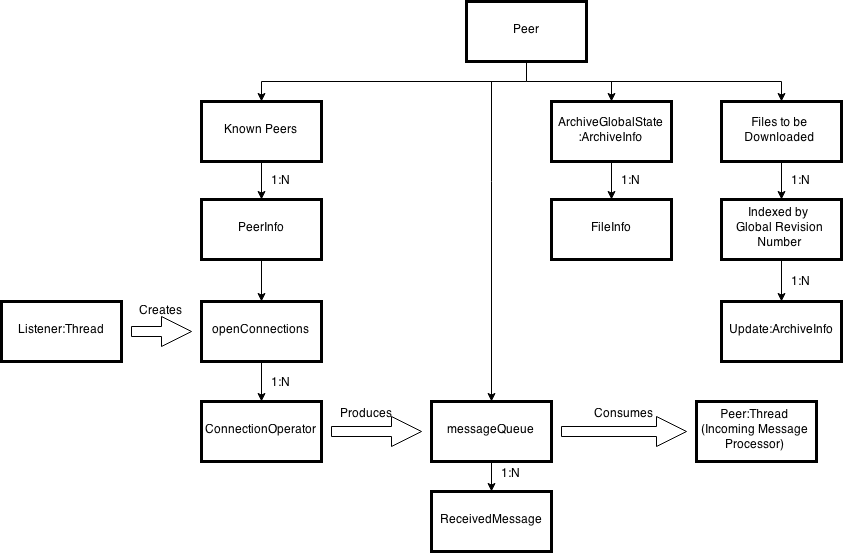
\includegraphics{strucs.png}
\caption{Figure 1: Main Program Data Structures}
\end{figure}

\subsection{Global and Local Archive
State}\label{global-and-local-archive-state}

The archive state structures each comprise the complete information
regarding a copy of the archive. Every peer maintains a global archive
state variable, which contains information about the most up-to-date
version of the archive. This includes which files are present, their
version numbers, size, and checksums. It can be thought of as the ideal
state of every peer's local copy. The second archive state variable, the
local archive state, is descriptive rather than proscriptive, like the
global archive state. It keeps track of the version information of the
locally-held copy of the archive. By comparing the global and local
archive state structures, Subscribers are able to ascertain which (if
any) files are missing or need updating, and make requests to other
peers for updates accordingly. Because the Publisher's copy of the
archive is by definition the authoritative one, it has no need of a
local archive state; or rather its local archive state \textbf{is} its
global archive state.

In order for each Subscriber's global archive state structure to be kept
up to date, the Publisher announces to every Subscriber upon the change
of a file in its archive copy. The file data itself is not sent
immediately, rather each Subscriber must make a request from the
Publisher, or another peer, for the files needed to bring their local
copy up to date. Subscribers joining or rejoining the network must
acquire fresh information about the global archive state, which may have
changed since their last time online.

\subsection{Known Peers}\label{known-peers}

Each peer maintains a list of peers which it has either ``seen'' (is or
has been connected to), or has been told about by another peer (after
requesting information about more peers from an already-known peer).
This list of peers is used when attempting to download or update the
local archive copy; rather than each Subscriber downloading from the
Publisher as in a Client-Server model, the bandwidth requirements for
each update are spread across the network using a peer-to-peer system,
where peers may download needed files from other peers who already have
the update. This list is populated by requesting other known peers for
information about others as mentioned above, or by receiving a
connection initiated by another peer.

Each peer may have zero or more open connections associated with it; in
other words, this peer may already be connected to another. Along with
these open connections, each peer may also have a pool of possible
connection addresses from which to create connections, should the need
arise.

While the list of connections provides a pool of possible addresses to
potentially connect to, there is no guarantee that a given peer can be
connected to. This may be due to network issues (such as firewalls or
routers), a lack of up-to-date information about addresses at which a
peer can be connected to, or because the peer itself is not online.

Distribackup's network communications have been designed to be
fault-tolerant against this; if any Subscriber is missing, then any
information requested of it can be requested from another. Subscribers
are relatively interchangeable from the perspective of other
Subscribers. Returning Subscribers can ask any and all Subscribers it
knows about from the last time it was online, and new Subscribers
joining the network must have the address of at least one peer already
on the network.

Connectivity issues with the Publisher are more difficult to work
around; when the Publisher is missing completely, no new updates can be
made to an archive contents, and some update information may be
completely unavailable -- for instance if the Publisher went offline
before completely syncing a newly-announced update to at least one other
peer. In the prototype created for this project, all that the remaining
Subscribers can do is bring the whole network as up-to-date as possible,
exchanging the most recent available file versions until there is
homogeneity. This is a relatively acceptable compromise, which ensures
relatively data security. However, in future versions of the protocol,
functionality may be added so that a new Publisher may be chosen from
existing Subscribers; the method for choosing, however, is as yet
undecided.

Finally, the network may find itself in a position of partial
connectivity; that is, peers can connect to some but not all others. In
this scenario, DNIEpr's design would ensure that no special re-routing
would need to take place; as long as each peer has one other peer it can
connect to, messages will still propagate (albeit more slowly) across
the network. In the current project prototype, peers retain no state
about which other known peers are or have become unreachable. Future
work could include researching whether passing connectivity information
to other peers, and remembering which information is true, would have
any benefit in terms of reducing wasted bandwidth through failed
connections.

\subsection{Received Message Queue}\label{received-message-queue}

\begin{itemize}
\itemsep1pt\parskip0pt\parsep0pt
\item
  a queue of enums which each represent incoming events
\item
  a single event handling thread deals with each event in order
\item
  each event enum will need info about it attached, like WHICH peer
  announced its exit
\item
  connection operators receiving bytes (which they then decode into
  messages) will add to the queue
\end{itemize}

\chapter{Process Description}\label{process-description}

This chapter describes, in structured English, the actions taken by each
peer in various situations encountered during normal operation.

\section{Non-New Peer Joins Network}\label{non-new-peer-joins-network}

This situation occurs when a peer, which has been previously seen by
some or all peers in the network, rejoins network after a period of
absence. The actual period of time the peer was not active on the
network does not affect the action taken; one archive's contents may
change completely in 5 minutes, while another may remain static for
years.

\begin{itemize}
\item
  Peer checks integrity of file tree by checking against stored values
  of size, name, checksum for every file

  If there are discrepancies: and we're a Subscriber: see Subscriber
  Loses Some Or All of Local Copy. or if we're the Publisher: see
  Publisher Has Updates else no discrepancies: If we're a Subscriber:
  check with Publisher about new peers and file updates Or if we're the
  Publisher: check if any new Peers have joined via DHT or otherwise
\end{itemize}

\section{Upon a file change}\label{upon-a-file-change}

\begin{verbatim}
FileSystemWatcher alerts main thread of file change

```
if a file has been deleted:
    if file is confirmed to exist on other mirrors,
    and is identical on other mirrors:
        then a deletion announcement is sent through overlay network to other mirrors

if a file is added:
    rsync is used to find which mirrors don't have the file
    file is sent via p2p implementation to any mirrors which don't have the file (or a piece of it)
    
if a file is updated:
    rsync diffs these changes against copies on other mirrors
    differing chunks are sent via p2p implementation
\end{verbatim}

```

\section{New Subscriber Joins
Network}\label{new-subscriber-joins-network}

\begin{enumerate}
\def\labelenumi{\arabic{enumi}.}
\itemsep1pt\parskip0pt\parsep0pt
\item
  New subscriber S connects to publisher P on P's listening port
\item
  P and S exchange version numbers; if they don't match, disconnect and
  warn users at P and S
\item
  P and S exchange UUIDs. These will later serve as keys, mapping to
  PeerInfo objects.
\item
  S sends P PeerInfo of itself, containing relevant info (see message
  binary spec)
\item
  P sends S a File Tree Status object, informing S of the latest
  versions
\item
  P sends S a PeerInfo List of the peers it knows about (hopefully all
  of them)
\item
  S Greets peers it heard about from P, sends File Requests for
  files/versions it doesn't have
\item
  Peers send back list of requested pieces they have/are able to send
\item
  S chooses best peer to download each file or piece from, based on
  speed or other metrics
\item
  Some kind of sanity check is performed to make sure everything went OK
\end{enumerate}

\section{Publisher Announces Update}\label{publisher-announces-update}

\begin{enumerate}
\def\labelenumi{\arabic{enumi}.}
\itemsep1pt\parskip0pt\parsep0pt
\item
  P announces to all known peers the changed file revision numbers
  (partial file Tree state info)
\item
  If P has any data about bandwidths of various subscribers, the files
  are sent to the fastest first, to maximise the number of peers that
  can supply the file. If not, a random subscriber is chosen
\item
  Every time a subscriber finishes downloading a file, it announces to
  peers it hasn't heard the same announcement from.
\item
  For every subscriber still downloading the file, requests are made for
  that file to those who have it.
\item
  Data is gathered by every peer about speeds during the transfer
\end{enumerate}

\section{Subscriber Exits Gracefully}\label{subscriber-exits-gracefully}

\begin{enumerate}
\def\labelenumi{\arabic{enumi}.}
\itemsep1pt\parskip0pt\parsep0pt
\item
  Exit announcement is made to all known peers
\item
  Any transfers this subscriber has in progress are finished, or if
  they'll take too long (which is how long?), cancelled
\item
  Sockets etc are closed
\item
  Peers set their record for this Peer as `offline'
\end{enumerate}

\section{Subscriber is in the Middle of Downloading a FileInfo, When a
New Version is
Announced}\label{subscriber-is-in-the-middle-of-downloading-a-fileinfo-when-a-new-version-is-announced}

\subsection{Publisher Leaves Network
Gracefully}\label{publisher-leaves-network-gracefully}

the publisher may intend for the files to remain static, so a new
publisher won't be elected unless (good\_reason). any new peer which
joins by contacting a peer will be brought up to date by the network
(version check, file list exchange, sync files with p2p) once (if) it's
implemented, peers may also find the network by DHT.

\section{Subscriber Exits
Ungracefully}\label{subscriber-exits-ungracefully}

Any peers with existing open connections to this Subscriber are
immediately notified by Java's Sockets API that the connection has been
closed suddenly.

\section{Publisher Exits}\label{publisher-exits}

\begin{enumerate}
\def\labelenumi{\arabic{enumi}.}
\itemsep1pt\parskip0pt\parsep0pt
\item
  Peers exchange information about the latest updates they've seen,
  until they are all in agreement.
\item
  Updates are requested from one another, until all Subscribers have
  most recent available versions of files
\item
  The network awaits the return of the Publisher; otherwise no changes
  are made or exchanged
\end{enumerate}

\section{Subscriber Experiences Data Loss; Subscriber's Copy is
Erroneously
Edited}\label{subscriber-experiences-data-loss-subscribers-copy-is-erroneously-edited}

\begin{enumerate}
\def\labelenumi{\arabic{enumi}.}
\itemsep1pt\parskip0pt\parsep0pt
\item
  The user is warned that this is a bad idea: any changes will be
  overwritten. If they want to edit the files, then they should make a
  copy
\item
  Procedure for 1 out-of-date peer is followed
\item
  Request more peers and files from all known peers
\item
  Subscriber announces its loss
\end{enumerate}

\chapter{Testing}\label{testing}

Quantitative, functionality-based tests were performed in order to
ascertain whether the program functions in the manner intended.

\section{Testing correct functioning of
DNIEPr}\label{testing-correct-functioning-of-dniepr}

In order to ensure that the underlying translation functionality between
DNIEPr's data types and binary arrays worked correctly, a testing suite
was created run regularly against the DNIEPr library.

The tests involved creating random (but valid) input data for each given
data type, then converting it to binary and back again. The
pre-conversion and post-conversion values were tested for equality. If
the values did not match, then both pre-conversion and post-conversion
values were printed to screen, to assist with debugging.

\section{Software Portability}\label{software-portability}

\begin{verbatim}
* HOW cross platform? (Linux, Windows, Android...)
\end{verbatim}

\section{Correct Syncing of Files}\label{correct-syncing-of-files}

\begin{itemize}
\itemsep1pt\parskip0pt\parsep0pt
\item
  Is the system resistant to attack?

  \begin{itemize}
  \itemsep1pt\parskip0pt\parsep0pt
  \item
    random peers going down
  \item
    Publisher impersonation/spoofing
  \item
    archive status misinformation
  \end{itemize}
\end{itemize}

\chapter{Evaluation}\label{evaluation}

In order to evaluate whether the implemented prototype successfully
fulfilled the goals of the original design, a qualitative evaluation was
performed.

The main competitors to to this software are Bit-Torrent Sync and
DropBox, due to the similarity of parts of each project's functionality.
Although the primary intended use of this software is for backup, these
technological similarities along with the popularity of DropBox will
mean they will offer direct competition.

As such, some the project was compared against each piece of software,

\begin{itemize}
\itemsep1pt\parskip0pt\parsep0pt
\item
  How well does the system cope with sudden changes in network topology?
\item
  How efficient is it? (bandwidth usage, processor \& memory usage)
\item
  completeness of the API

  \begin{itemize}
  \itemsep1pt\parskip0pt\parsep0pt
  \item
    lack of ambiguity
  \end{itemize}
\end{itemize}

\section{Results of the evaluation}\label{results-of-the-evaluation}

\chapter{Conclusions}\label{conclusions}

A need was identified in domestic environments for robust long-term
backup software which required as little user-intervention as possible;

\section{Future Work}\label{future-work}

It was necessary to streamline the functionality implemented in the
prototype due to time constraints, in order to finish the core file
watching and transfer functionality. This section talks about extensions
to the submitted prototype that could be added during future development
cycles.

\subsection{Android Client}\label{android-client}

\subsection{Windows Client
Improvements}\label{windows-client-improvements}

\subsection{Multiple Archive Networks}\label{multiple-archive-networks}

\subsection{Change of Publisher}\label{change-of-publisher}

\subsection{Encryption/Authentication}\label{encryptionauthentication}

Encryption, although not initially a high priority in the system
prototype, this can be broken into 3 sub-areas; PGP is a good candidate
for providing any of these. All of these, though especially the first
two, are highly desirable.

\subsubsection{Transfer encryption}\label{transfer-encryption}

Preventing digital wire taps from snooping on data in-transit is
extremely important, especially given the use of a public network (the
internet) as the transmission medium.

\subsubsection{Authentication}\label{authentication}

Prevent attackers from joining the network without permission, and
prevent malicious peers claiming to be the Publisher from making
erroneous updates.

\subsubsection{Local storage encryption}\label{local-storage-encryption}

Focus on interfacing with existing file-system encryption technology
here. Less important for backup software, as encryption always
introduces the risk that the access method (such as a password or key)
will be lost over time.

\subsection{Compression}\label{compression}

\subsection{Better File Transfer Load Balancing
Algorithm}\label{better-file-transfer-load-balancing-algorithm}

\subsection{Graphical or Web User
Interface}\label{graphical-or-web-user-interface}

\subsection{Persistent Peer IDs}\label{persistent-peer-ids}

\subsection{Web-visible files}\label{web-visible-files}

hosted web pages and web links to files

\begin{itemize}
\itemsep1pt\parskip0pt\parsep0pt
\item
  Version control for managed files

  \begin{itemize}
  \itemsep1pt\parskip0pt\parsep0pt
  \item
    Likely to be implemented using Git
  \end{itemize}
\item
  Multiple networks, multiple folders in each

  \begin{itemize}
  \itemsep1pt\parskip0pt\parsep0pt
  \item
    This could get complex for the user very quickly
  \end{itemize}
\item
  Human-readable anonymous peer IDs

  \begin{itemize}
  \itemsep1pt\parskip0pt\parsep0pt
  \item
    map IP address of a peer to a country,
  \item
    then hash the peer's UUID to choose a name from a list specific for
    that country
  \end{itemize}
\end{itemize}

\begin{thebibliography}{9}

\bibitem{fosdem15rice} Dave Rice "Enabling video preservation through open source", FOSDEM 2015 (https://fosdem.org/2015/schedule/event/enabling\_video\_preservation/) (accessed 19/03/2015, attended talk on 31/01/2015)

\end{thebibliography}

\end{document}
